\section{Bayesian Network}
The syntax of a Bayesian network is the following:
\begin{itemize}
    \item a set of nodes, one per variable
    \item a direct, \textbf{acyclic} graph
    \item a conditional distribution for each node given its parents.
\end{itemize}

It is a Probability Graphical Model (PBG). We use a Condition Probability Table (CPT) to represent causes and effects. Given the parents of the node $X_{i}$, he is independent from all the other variables. I only have to express $P(X_{i} | Parents(X_{i})$.

Consider a set of rules: $A\xrightarrow{}C$, $B\xrightarrow{}C$, $B\xrightarrow{}E$, $C\xrightarrow{}E$, $C\xrightarrow{}D$. Instead of having $P(A, B, C, D, E)$, I can use: $P(A)$, $P(B)$, $P(C|A,B)$, $P(E|B,C)$ and $P(D|C)$. We can use the chain rule to calculate probabilities:
\begin{figure}[H]
    \centering
    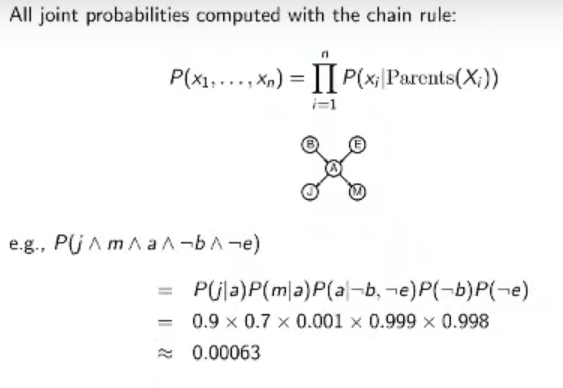
\includegraphics[width=7cm]{images/BayesianNetwork/Bayesian_Networks.png}
    \caption{Caption}
    \label{fig:Bayesian_networks}
\end{figure}

We can use the parameters $\Theta = <\Theta_{1}, \dots, \Theta_{n}>$ and calculate the inference. In machine learning we are interested in learning these parameters given a dataset.

If we can observe every variable it is easy since we can count the number of times that each variable is true/false and infer probabilities:
\begin{equation}
    P(A=1 | B = 0) \approx \frac{|\{d_{k} = \langle a_{k}, x_{k}, \dots\rangle \}| a_{k} = 1 \And x_{k} = 0|}{|\{d_{k} | x_{k} = 0|\}}
\end{equation}

If we have an unknown variable $X$ we can define $\Theta_{1} \dots \Theta_{n}$ as $P(X = 0) = \Theta_{0}$, $P(A = a_{1} | X = 0) = \Theta_{1}$, $P(A = a_{1} | X = 1) = \Theta_{2}$, $P(B = b_{1} | X = 0) = \Theta_{3}$, $P(B = b_{1} | X = 1) = \Theta_{4}$, $\Theta = \langle \Theta_{0}, \Theta_{1}, \Theta_{2}, \Theta_{3}, \Theta_{4} \rangle$ and use EM algorithm to maximize $\Theta$ from $D = \{(a_{1}, b_{1}), \dots, (a_{k}, b_{k})\}$.

Estimation:
\begin{equation}
    \begin{multlined}
        P(X = x_{j}) = \frac{1}{N} E [\hat{N}(X = x_{j})] \\
        P(A = a_{j} | X = x_{j}) = \frac{E[\hat{N}(A = a_{j}, X = x_{j})]}{E[\hat{N}(X = x_{j}]}
    \end{multlined}
\end{equation}
Maximization:
\begin{equation}
    E[\hat{N}(\cdot)] = E\left[\sum_{k}I(\cdot|d_{k})\right] = \sum_{k} P(\cdot | d_{k})
\end{equation}